\section{Macro-genre Analysis Strategies: Three Variations}
There are three standard analytic approaches in the quantitative sociology of taste. All begin from the same starting point, however, a rectangular (two-way, two-mode) matrix ($A$) with (usually) people $\left(P1, P2, P3,\ldots P_N
\right)$ in the rows and cultural genres $\left(G1, G2, G3,\dots G_K\right)$ in the columns. As noted at the outset, the {\em ways} of the matrix are the number of dimensions, and the {\em modes} of the matrix are the number of entity types for which data have been collected \citep{borgatti_everett97}. In the usual case, we have two-way, two-mode (people and genres) data \citep{lizardo18}. The goal of the analysis is to learn some kind of \textit{classification} of either the people or the genres (or both) from the data. This setup is shown in figure~\ref{fig:reg_approaches}. 

In this (toy) example, we have five people and four genres. Each cell in the $A_{PG}$ matrix equals one when person $P$ engages (e.g., likes, listens) genre $G$; otherwise, it equals zero. Reading across the rows, we find each person's pattern of cultural choices \citep{peterson83}. So we learn that person 1 engages genres 2 and 3, and person 3 engages all four genres; maybe they are an ``omnivore''. Reading down each column, we find the popularity of each genre or the number of people who engage in it. So we learn that genre 4 is engaged by four people (2, 3, 4, and 5), and genre 2 is only engaged by two people (3 and 4). Maybe genre 4 is a ``popular'' genre, and genre 2 is a ``niche'' genre \citep{lizardo18}. 

Of course, researchers usually want to go beyond describing the cultural choice patterns of individual people or the audience distribution of each genre. Instead, researchers use specific data reduction techniques to classify either the genres, the people or both. Let us consider each of these possibilities in turn.

\begin{figure}[ht!]
 \centering
 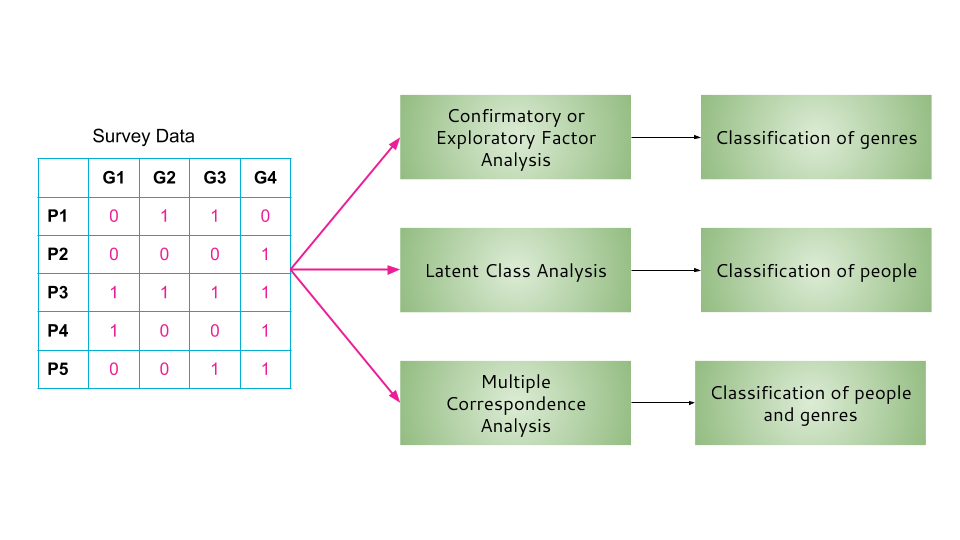
\includegraphics[width=1.0\textwidth]{Figs/Regular/reg-approaches.png}
 \caption{Three approaches to classifying survey data on cultural tastes.}
 \label{fig:reg_approaches}
\end{figure}

\subsection{Classifying Genres: Factor Analysis (FA)}
One thing that we could do with the (real) data described earlier is to attempt to come up with a classification of musical genres. Recall that in these data, we have $2263$ people in the rows and $20$ (musical) genres in the columns. One well-established and long-pedigreed technique allowing us to come up with clumps of the variables in a person-by-variables table (with a long history in psychometrics) is Factor Analysis (FA). This method uses the genres as variables and relies on a factorization (hence the name) of the correlation or covariance matrix between these variables to extract a smaller number of dimensions. We can then classify each genre based on their loading (e.g., correlation with) each dimension extracted. The output of such an exploratory factor analysis of the SSI 2012 data, featuring a four-factor solution, is shown in figure~\ref{fig:efa}. 

\begin{figure}[ht!]
 \centering
 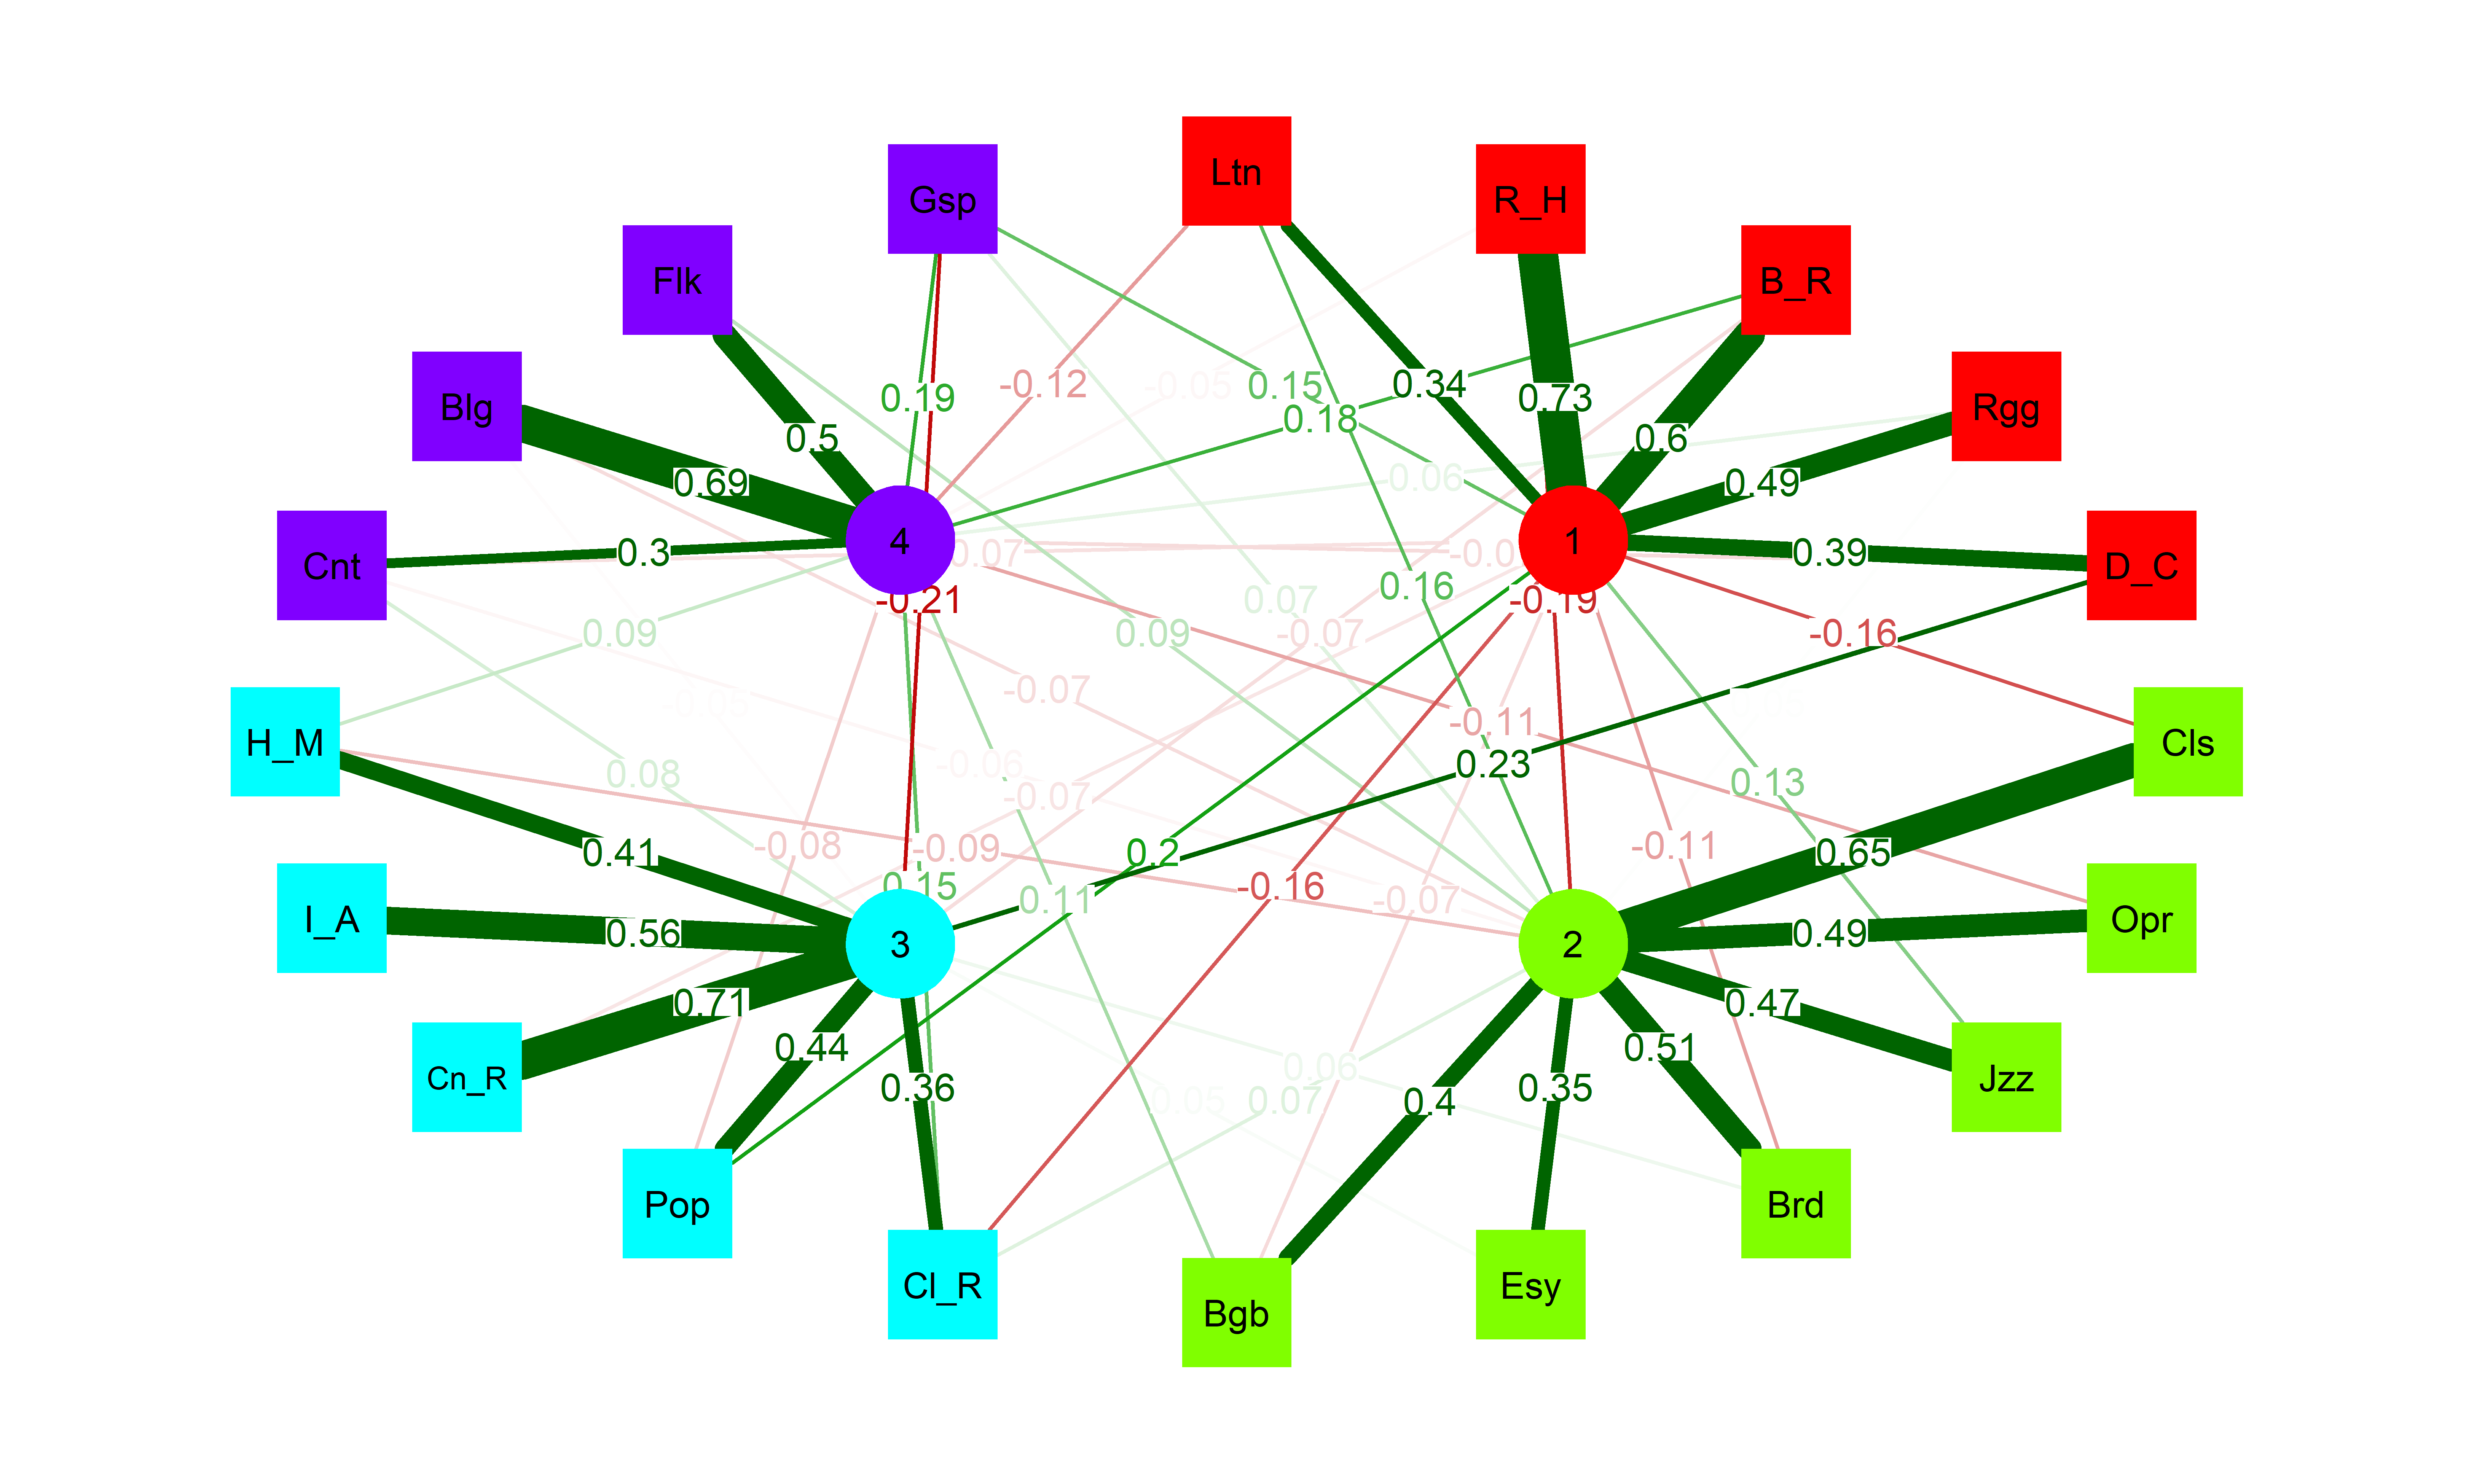
\includegraphics[width=1.0\textwidth]{Figs/Regular/genre-efa-regular.png}
 \caption{\footnotesize Point and line plot of exploratory factor analysis results (four-factor solution) of the musical taste data. Positive loadings between each factor (circles) and each of the genres (squares) shown as green edges. Negative loadings shown as red edges. Edge width is proportional to magnitude. Node labels should be read as follows. Factor 1 (red Nodes): Ltn (Latin/Spanish), R\_H (Rap/Hip Hop), B\_R (Blues and R \& B), Rgg (Reggae), D\_C (Dance/Club); Factor 2 (green nodes): Cls = Classical, Opr = Opera, Jzz = Jazz, Brd = Broadway Musicals, Esy = Easy Listening, Bgb = Big Band, Factor 3 (teal nodes): Cl\_R = Classic Rock/Oldies, Pop = Pop/Top 40, Cn\_R = Contemporary Rock, I\_A = Indie/Alternative, H\_M = Hard Rock/Heavy Metal; Factor 4 (purple nodes): Cnt = Country, Blg = Bluegrass, Flk = Folk, Gsp = Gospel.}
   \label{fig:efa}
\end{figure}

How do we interpret these pattern of results? One approach, for instance followed by \citet{vaneijck01}, is to inspect the factor loadings as indicating a classification of genres according to a higher order principle (e.g., logics or discourses); namely, a set of ``meta-genres.'' The results of the factor analysis is broadly consistent with such a hypothesis. For instance, factor 3 groups all the ``rock and pop'' related genres, and factor 1 groups together a related set of ``Afro-pop'' genres such as Rap, Reggae, and R\&B. Together, they might constitute a discourse of ``fun.'' Factor 2 groups together all the usual ``highbrow'' genres, such as Classical, Opera, and Jazz, reflecting a more austere ``art'' discourse. Finally, the genres loading highly on factor 4 such as Country, Bluegrass, and Folk may reflect a more down to earth ``folk'' discourse linked to roots authenticity \cite{vaneijck01}. 

\subsection{Classifying the People: Latent Class Analysis (LCA)}
Another approach relies not on classifying the genres, but classifying the people. The idea here is to rely on the fact that each person produces a ``response pattern'' (a ``pattern of cultural choice'' in Richard Peterson's \citeyear{peterson83} classic locution).The pattern corresponding to a person ($P_i$) is thus the vector of zeros and ones corresponding to their row in the matrix shown in Figure~\ref{fig:reg_approaches}. The idea is that we can then (probabilistically) clump people into classes based on how similar these patterns are. People with similar patterns end up in the same clump; people with dissimilar patterns end up in different clumps \citep{chan_goldthorpe07, tampubolon2008revisiting}. One well-established and equally long-pedigreed technique that allows us to group people into clumps in a person by (categorical) variables table (with a long history in sociology, marketing and related fields) is Latent Class Analysis (LCA). 

\begin{figure}[ht!]
 \centering
 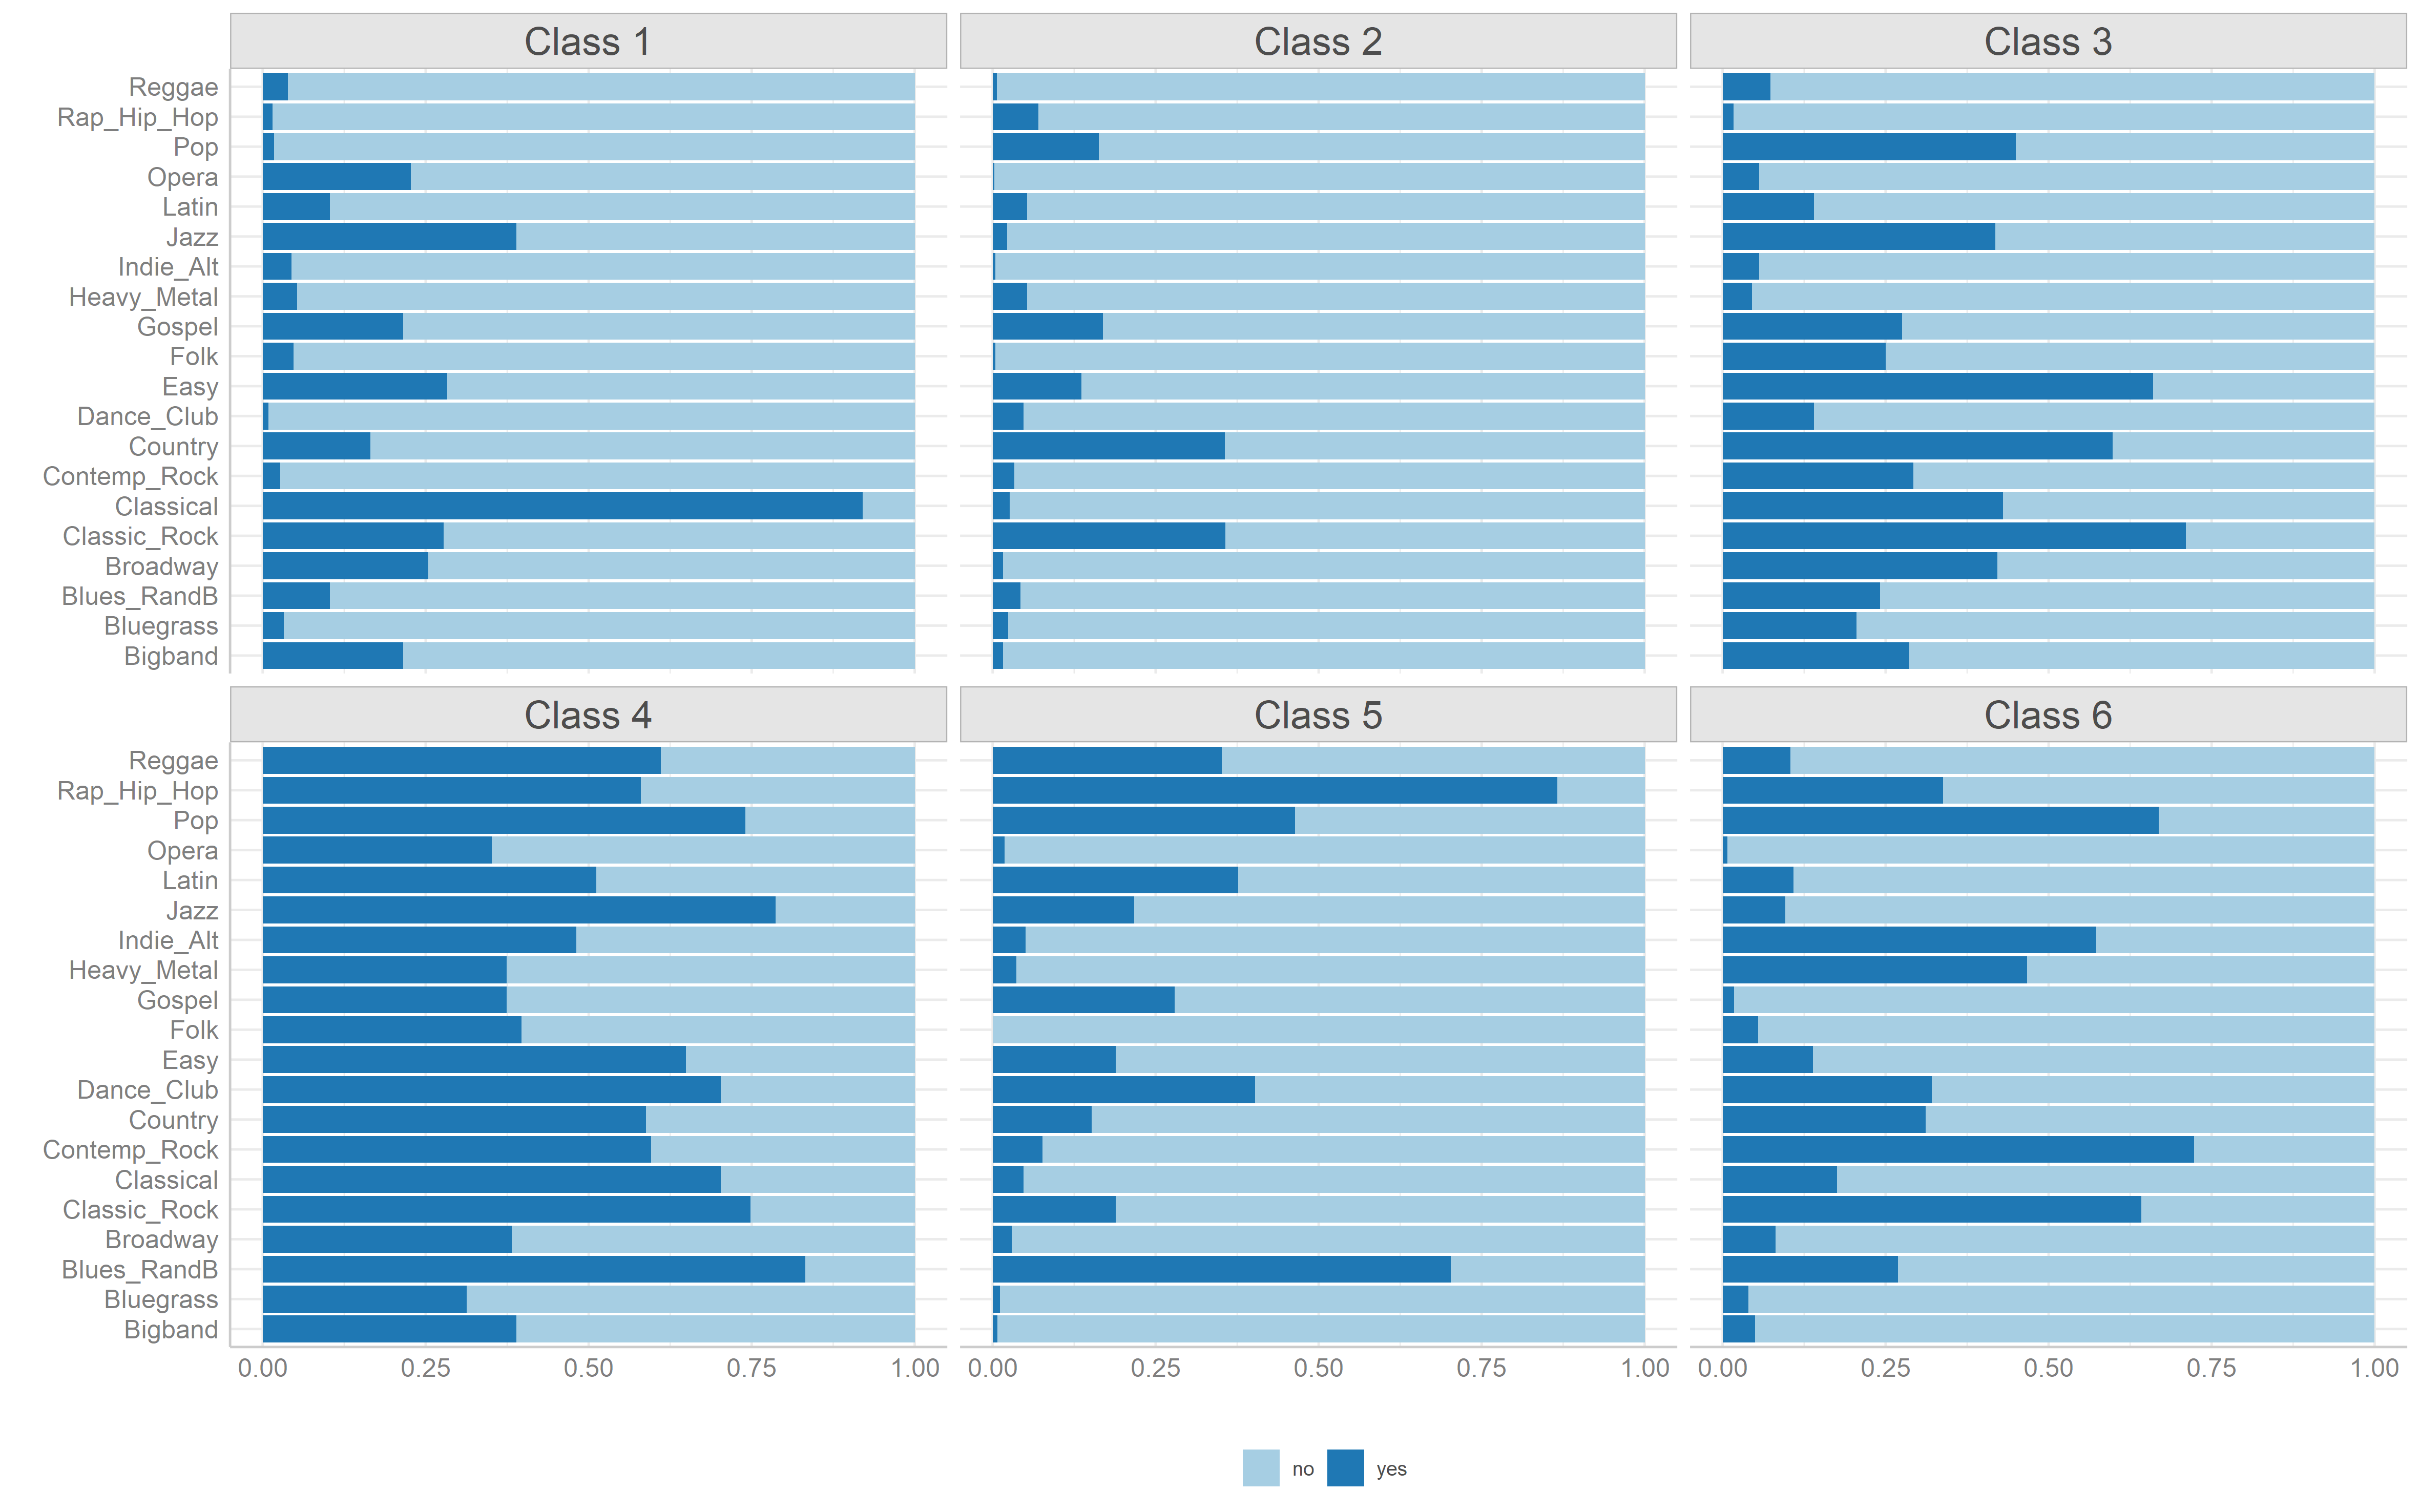
\includegraphics[width=1.0\textwidth]{Figs/Regular/genre-lca-regular.png}
 \caption{\footnotesize Stacked bar plot showing the proportion of people (shown in the x-axis) engaging ("yes" in dark blue) and not engaging ("no" in light blue) each genre (shown in the y-axis) by latent class assignment (plot panels).}
  \label{fig:lca}
 \end{figure}
 
The main output from an LCA is an $m$-dimensional vector (where $m$ is the number of latent classes requested) assigning each row $i$ of the data matrix (in this case the people) a probability of belonging to the $j^{th}$ latent class. Because memberships are mutually exclusive (each person can only belong to one latent class), these probabilities have to sum to $1.0$. This means that, if the solution fits the data well, one of the probabilities in the vector will be much larger than the others (e.g., $m_{ij} > 0.90$). We can then we can assign each person to the class they have the largest probability of belonging to. Once we have assigned each person to a class, we can go back to the data, and see how the clumps of people assigned to different classes differ in their cultural choice patterns. The output of such an exploratory latent class analysis applied to the same data as before, and featuring a six-class solution, is shown in figure~\ref{fig:lca}. 

How do we interpret these pattern of results? The usual approach in the sociology of taste, exemplified by \citet{chan_goldthorpe07} and \citet{tampubolon2008revisiting}, is to use the conditional probabilities of engaging genre $G$ given that a person belongs to class $m$ (shown in the separate panels of figure~\ref{fig:lca}) to baptize the classes with a given name. Thus, information from the genres (whether given by previous research, theory, or intuition) can help us make sense of what each of the people clumps means. For instance, we may find that one class of people (in this case class 4) has relatively high probabilities of engaging {\em all} genres. Maybe they are ``omnivores'' \citep{peterson_kern96}. Others, only engage have a high probability of engaging a couple of genres like Country and Classic Rock/Oldies (Class 2); maybe they are ``univores'' \citep{peterson92}. Some univores (like Class 1) just engaging very fancy, traditionally high-status genres like Classical; others (like Class 5) specialize in ``Afro-Pop" genres like Rap/Hip Hop and R\&B, while others (like Class 6) gravitate toward Contemporary Rock, Pop, Indie and Alternative music. 

We could further investigate the demographic composition of each class, by for instance, fitting a regression model for categorical response variables with multiple modalities (e.g., like the Multinomial Logit model) in the ``three-step'' approach \citep{bakk2013estimating}, or doing everything in one-step (letting the classes be affected by exogenous covariates, as with \citet{tampubolon2008revisiting}). We could then examine hypotheses about whether omnivores are young and educated, highbrow univores are old, Country/Oldies univores live mostly in the American South, Afro-Pop univores are more likely to be young and non-white and so forth (fancier approaches would do the class assignment and the regression model in a more efficient single step, but it is the same idea). 

\subsection{Classifying the People and the Genres: Multiple Correspondence Analysis (MCA)}
Finally, we may be interested in a technique that allows for the simultaneous classification of the people and the genres. The go-to technique for this job is Multiple Correspondence Analysis (MCA). Correspondence Analysis and related techniques have as old and storied histories as FA and LCA, but for a long time remained a well-kept secret (for English speakers) ensconced in multi-volume French mathematical monographs written by Jean-Paul Benz\'{e}cri and collaborators. 

Today the situation is different. MCA has now been fully introduced and extended in various anglophone monographs and collections \citep{leroux_rouanet04, greenacre_blasius06}, and algorithms implementing the basic mathematical ideas available in the standard statistical packages \citep{le_etal08}. Because of this, and very much ironically, while MCA (and not regression FA, or LCA) could be considered one of the {\em first} techniques that reinvigorated the modern empirical study of taste in sociology (figuring prominently in Pierre Bourdieu's \citeyearpar{bourdieu84} field-defining classic \emph{Distinction}), it has not been until recent that the method has begun to be used widely \citep[see][among many others]{flemmen_etal18, roose_etal12, savage_gayo11}.  
 \begin{figure}[ht!]
 \centering
 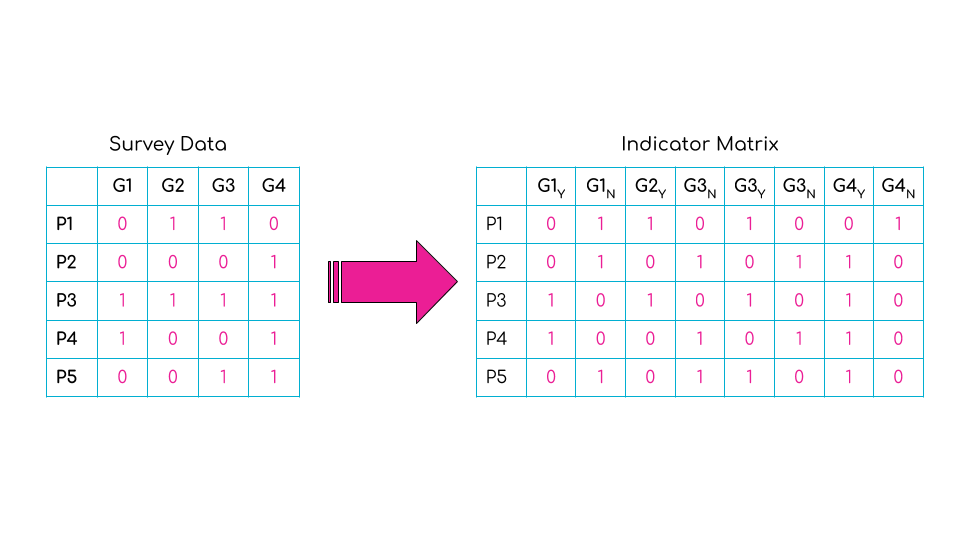
\includegraphics[width=1.0\textwidth]{Figs/Toy/mca-toy-ex.png}
 \caption{\footnotesize Transformation of original data matrix of people by genres, to an indicator matrix of people by genre-modality.}
  \label{fig:mca-toy}
 \end{figure}
 
 How does MCA work the magic of providing us with a simultaneous classification of people and genres? The trick, revealed in Figure~\ref{fig:mca-toy} using our running toy example, is to transform the original two-mode data matrix into an indicator matrix. In the indicator matrix, there is a column not for each variable (like in the original two-mode data) but for each {\em category of each variable} (these are usually called ``modalities'' in MCA-speak \citep{leroux_rouanet04}). Each variable has two categories in our toy case (and our real data). So we go from a 5 $\times$ 4 matrix to a 5 $\times$ 8 one (see Figure~\ref{fig:mca-toy}). Each genre $G$ column splits into two columns, $G_Y$ and $G_N$, and we put a one in the corresponding cell of the matrix under column $G_Y$ if the individual engages (e.g., likes, listens) to the genre. If the individual does not engage the genre, we put a one under the $G_N$. 
 
 The singular value decomposition (a kind of ``factor analysis for matrices'') of a suitable transformed version (each cell entry weighted by the row and column marginal sum) of the indicator matrix yields scores for each row and each column (both the "yes" and "no" answers to engaging the genre in our toy example) along many ``dimensions'' (also called ``axes'' or ``principal components''). Like in FA, the dimensions are ordered so that the first captures the closest representation of the original matrix (in the least squares sense), the second captures the best representation of the stuff left over, and so forth. The scores on each dimension are orthogonal and thus can be plotted in Euclidean space (e.g., of two dimensions). This can be seen as a low-dimensional representation of the original multidimensional matrix object. The clumps of people and genres thus emerge as clusters of (same-kind) entities that end up close together in this low-dimensional space. The capacity to visualize both people and especially the genres ``social space'' is one of the main appeals of the method \citep{greenacre_blasius06}, as evident in Bourdieu's \citeyearpar{bourdieu84} classic work. These scores are the main thing that MCA learns from the data. The output of such a multiple correspondence analysis of the data, featuring a four-factor solution, is shown in figure~\ref{fig:mca}. 
 
 \begin{figure}[ht!]
 \centering
 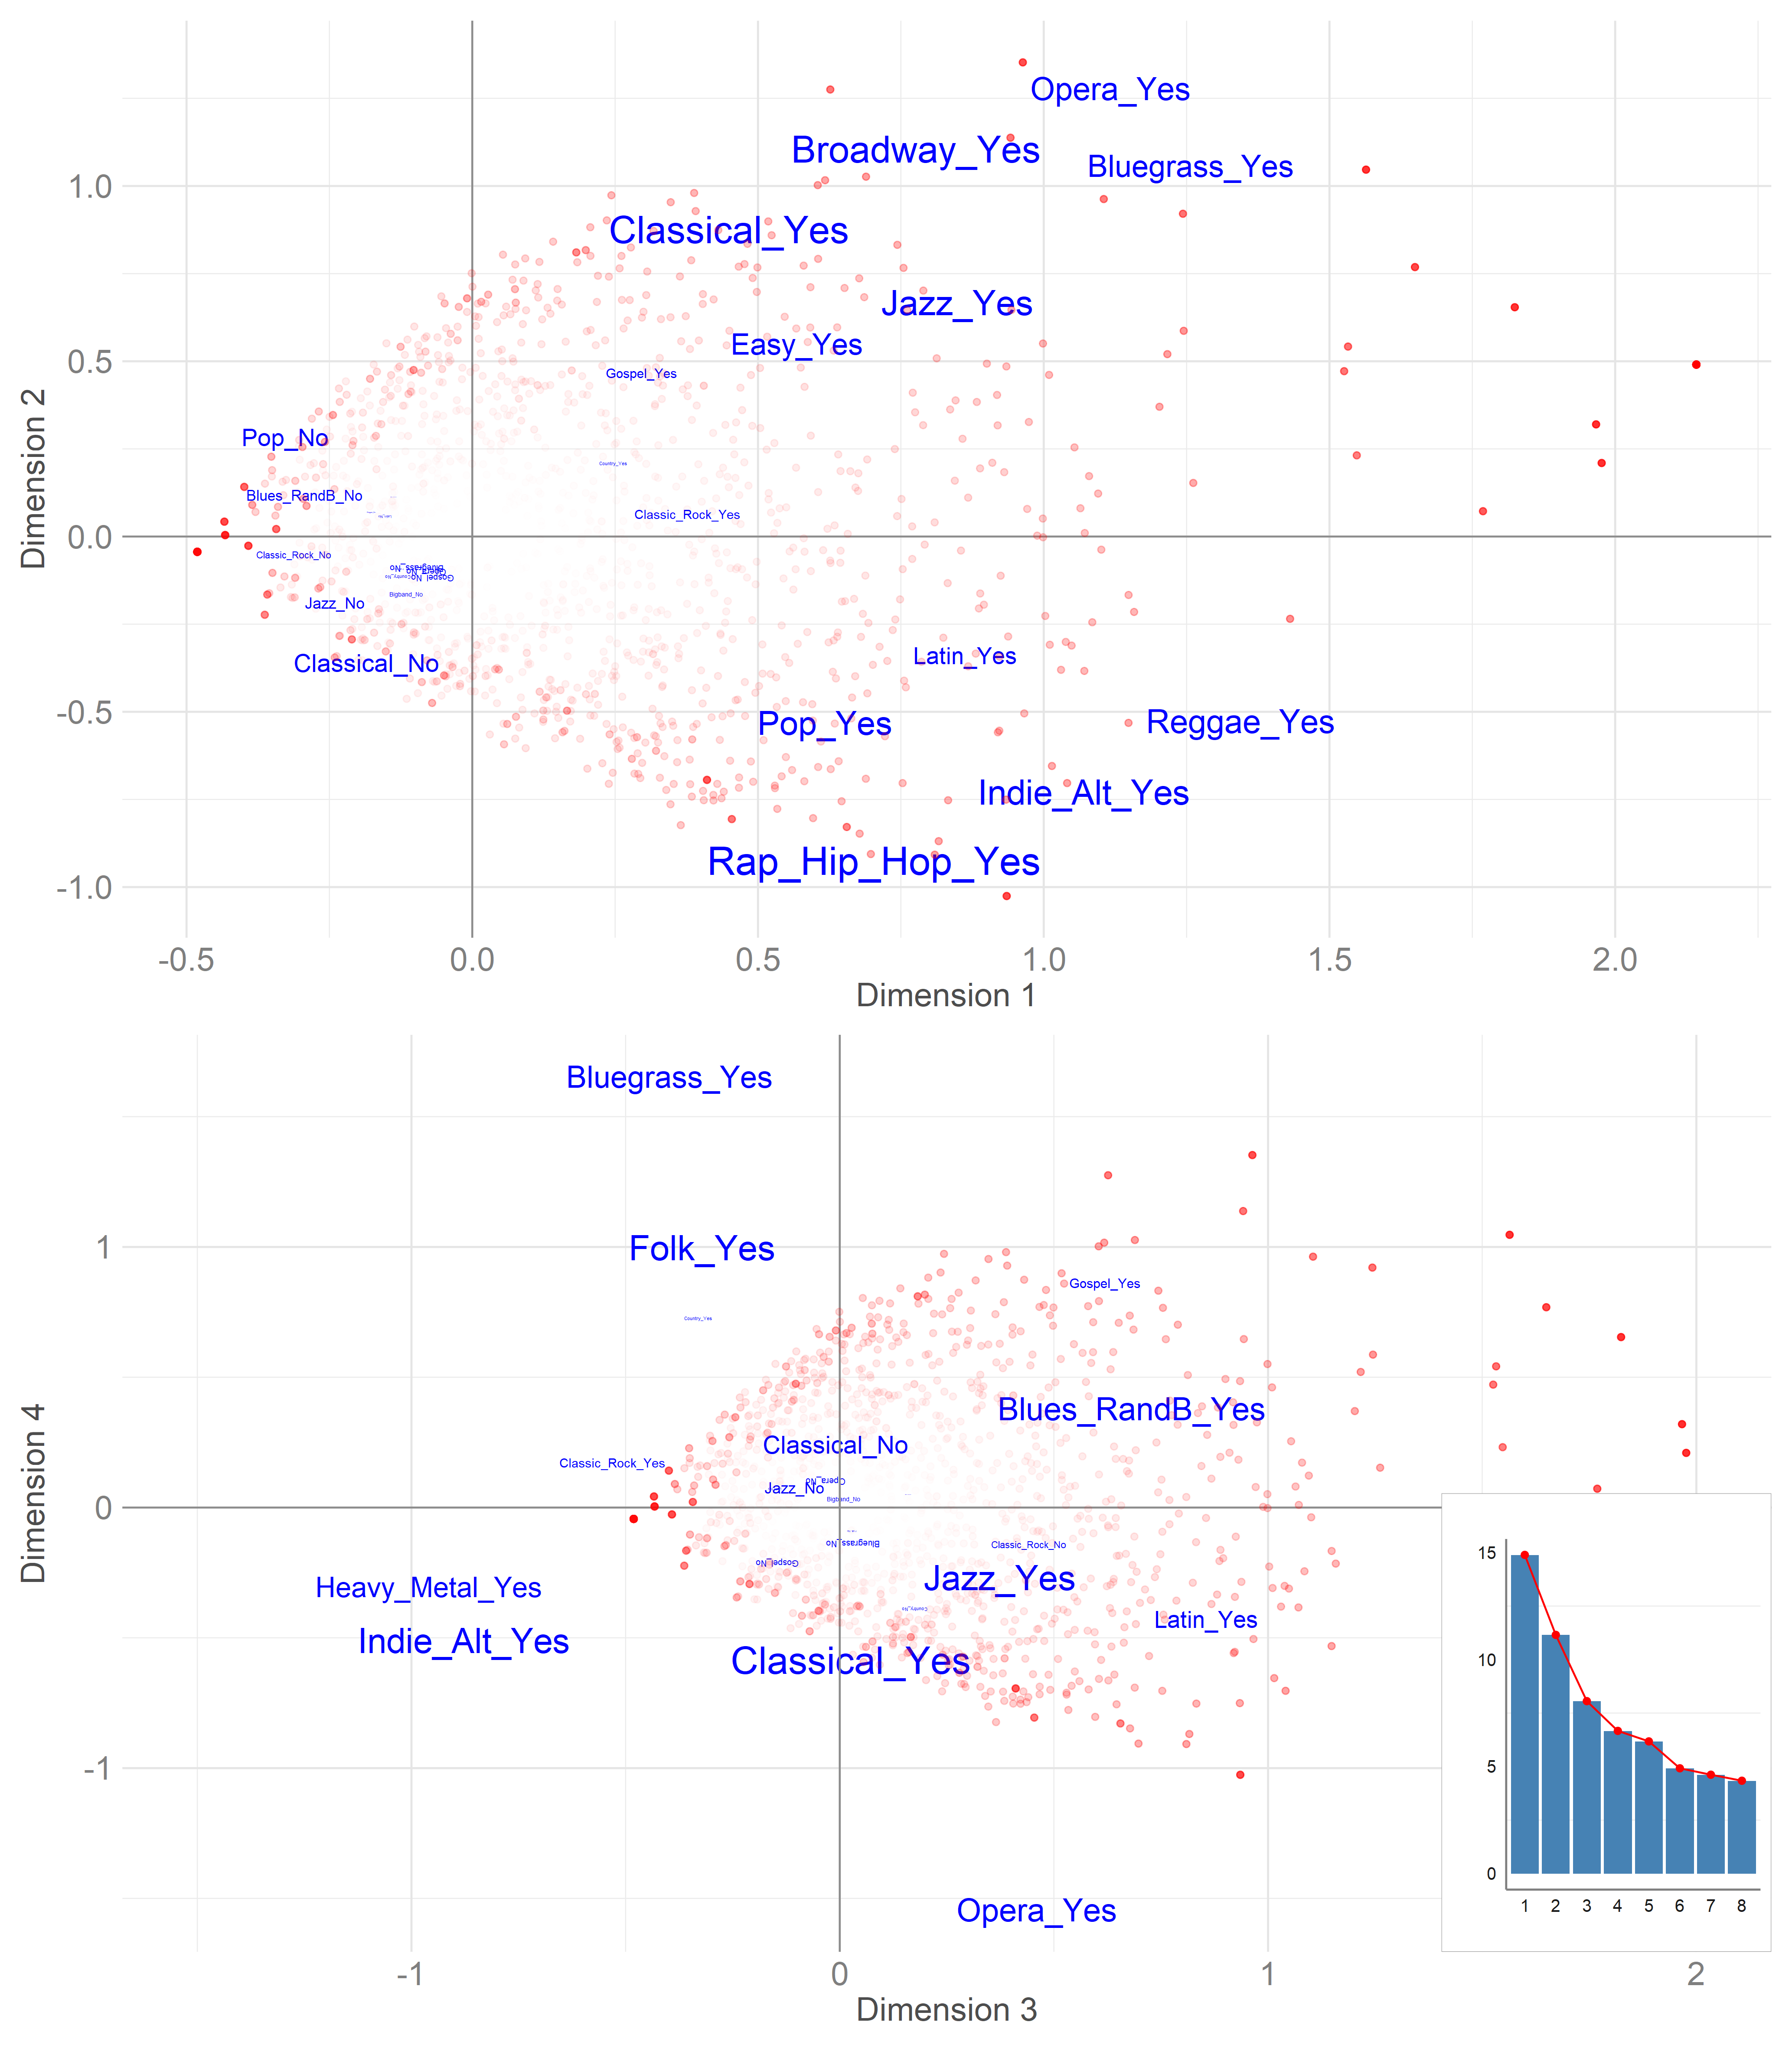
\includegraphics[width=1.0\textwidth]{Figs/Regular/genre-mca-regular.png}
    \caption{Multiple Correspondence Analysis (first four dimensions) of the musical taste data. Survey modalities (genre chosen: Yes/No) shown in blue text, ``cloud of individuals" shown as red points with shading proportional to the contribution. Inset plot (blue bars) show eigenvalues of first eight dimensions.}
    \label{fig:mca}
 \end{figure}
 
 How do we interpret these pattern of results? We can follow some of (many) recent papers that have used MCA to understand the link between people and genres \citep[e.g.,][]{roose_etal12}. As noted we can see the modalities that clump together along a given dimension as telling us something about what that dimension represents. So, looking at the horizontal (first) dimension of the left-hand side biplot (panel a), it is easy to see that all the "yes" modalities are to left of that horizontal dimension (indicating values greater than zero) and all the "no" modalities are to the right. So the main thing that the MCA picks up is a distinction between people who engage the genres and people who do not (actives versus abstainers). Note that the both people (the red dots forming the ``cloud of individuals'') and the genre modalities are distributed in a classic ``horseshoe'' pattern in this space, indicating that this first dimension is {\em ordinal}, separating people who engage many genres from those who engage none. This finding has been replicated repeatedly in many MCA analyses done on various cultural taste and participation data across dozens of countries.
 
 What does the second dimension tell us? Well, it seems like (looking at panel b) here, the usual distinction between fancy, high-status genres (with high positive scores at the top) and popular, industry, or just plain fun genres (with high negative scores at the bottom) reasserts itself. So ``net" of engagement, we find that engagers are partitioned across a highbrow/popular divide \citep{roose_etal12, flemmen_etal18}. Looking at genre clumps (really active engagement with genres clumps) in dimensions 3 and 4 reveals further insights. In fact, looking at how the genres and the people are distributed in this space, we can see that net of the quantitative distinction between engagers and non-engagers, and the broad binary genre distinction between ``traditional and popular'' what re-appears is the van Eijckian pattern differentiating of genres into four discourses or meta-genres: The same genre classification revealed by FA (see Figure~\ref{fig:efa}). Categories indicating engagement with (predominantly white-performer-dominated) rock genres clump together, engagement with Folk and Country genres clumps together, traditionally fancy genres clump together, and ``Afro-pop'' pop genres clump together. People are evenly distributed (in a nice circle) across all four quadrants of this space, indicating that these logics may be a powerful organizing principle of the ``musical taste field'' \citep{savage_gayo11} in the contemporary U.S.
 
More advanced applications of MCA would be beyond eyeballing the clumps and do some other things \citep{leroux_rouanet04}. For instance, since MCA produced scores along a multidimensional Euclidean space, this means that {\em distances} among each pair of elements of the same kind (people or genre engagement modalities) are defined. We can thus compute such distances and produce data (not eye) driven clumps using hierarchical clustering (with Ward's criterion) \citep{becue-bertaut_pages08}, an approach that was first developed by Benz\'{e}cri himself \citep{leroux_rouanet04}. We could also ``project'' categories (modalities) corresponding to people's demographic characteristics (e.g., by computing the average score in each dimension for people with e.g., a college degree, professional occupation, and so forth). We could even engage standard hypothesis testing, by for instance, figuring out if the mean score in Dimension 3 is statistically different for people who identify with different ethnoracial categories \citep{flemmen_etal18}.
 
\section{Getting out of the (Macro) Genre Bubble}
There is no question that the three approaches so far discussed, used to classify genres, classify people, or simultaneously classify people and genres, are the workhorses of the quantitative empirical study of taste today. All, by the same token, are vulnerable to the ``genre'' critique outlined in the introduction. For instance, both FA and MCA suggest that engagement with ``Opera'' or ``Classical'' is different from engagement with ``Rap'' or ``Country.'' These (macro) genres belong to different universes, discourses, or what have you \citep{vaneijck01}. But a critic of the genre concept can point to other types of qualitative and historical evidence collected on both people and genres, weakening our confidence in this conclusion \citep{lena2015relational}. All provide fodder for a version of the micro-genre or genre differentiation critique of traditional quantitative empirical work on the sociology of taste that does not collect sufficiently fine-grained information on cultural preferences. 

Notably, {\em what} technique you use (FA, LCA, MCA) does not really matter; from the micro-genre critique perspective, it is garbage in and garbage out. MCA will produce an ``opposition'' between macro-genres and even results that are consistent with techniques (such as FA) that are usually posed as enemies of MCA. The problem is that poor MCA (or LCA or any other method) only has the macro-genre-based categories to work with. Tasked with finding patterns using these data, the algorithm delivers, but what it delivers is, from the micro-genre perspective, misleading or only partially true results. 